
\section{Joint Finger-knuckle and Fingerprint Project}

\subsection{A Brief Summary of the Original Report}

The author of the technical report uses the hand-craft feature descriptor to extract finger knuckle and fingerprint features, and uses a very simple method to consolidate matching score by score level combination. Firstly, he uses the local feature descriptor based approach introduced in \cite{zheng20163d}, \cite{kumar2016personal} to extract finger knuckle template. In terms of fingerprint, the COTS (VeriFinger) \cite{verifinger} matcher can outperform NBIS \cite{watson2007user} and MCC \cite{cappelli2010minutia} on the fingerprint dataset result in using the commercial fingerprint matcher on the paper. At the last step, he uses Dynamic Match Score Consolidation method to get the final matching score $s_c$, as shown in Algorithm 1.

\begin{algorithm}[h!]
    \centering
    \renewcommand{\algorithmicrequire}{\textbf{Input:}}
    \renewcommand{\algorithmicensure}{\textbf{Output:}}
    \caption{Dynamic Match Score Consolidation}
    \begin{algorithmic}[1]
        \REQUIRE Match score: $s_k$ (finger knuckle), $s_f$ (fingerprint), \\
        Quality score: $q_k$ (finger knuckle), $q_f$ (fingerprint), \\
        Weight parameter $w$ ( $0 \leq w \leq 1$)
        \ENSURE Consolidated score $s_c$
        \IF{$q_k$ \textless 1 and  $q_f$ = 1}
        \STATE $s_c$ = $s_f$
        \ENDIF
        \IF{$q_k$ = 1and  $q_f$ \textless 1}
        \STATE $s_c$ = $s_k$
        \ENDIF
        \IF{$q_k$ \textless 1 and  $q_f$ \textless 1}
        \STATE $s_c$ = 0
        \ELSE
        \STATE{$s_c$ = $w \times s_k + (1-w) \times s_f$}
        \ENDIF
        \RETURN $s_c$
    \end{algorithmic}
\end{algorithm}

\textcolor{red}{\subsection{What I Have Done}}
\subsubsection{Using Pre-trained RFN model}

\begin{figure*}[ht!]
    \centering
    \subfloat[]{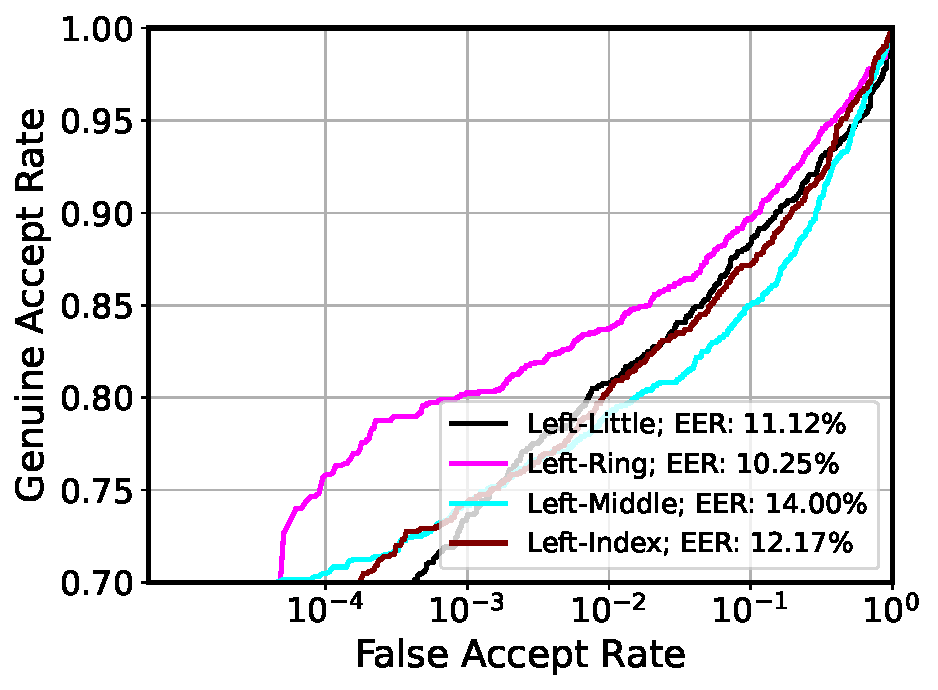
\includegraphics[width=3in]{Figure/09-09-2022/left-roc.pdf}}
    \subfloat[]{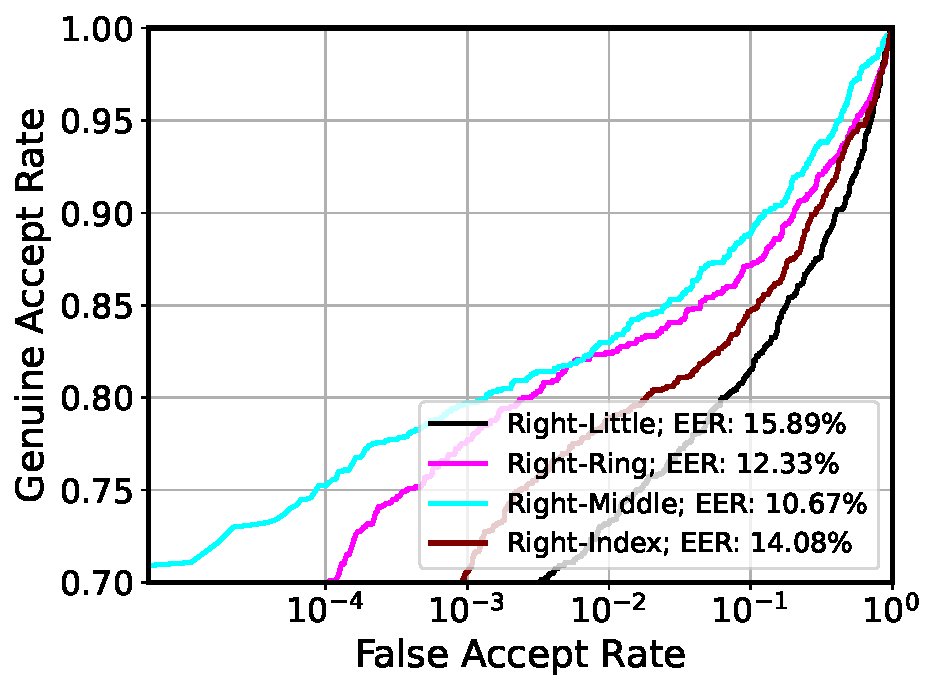
\includegraphics[width=3in]{Figure/09-09-2022/right-roc.pdf}}
    \caption{Comparative ROC curve from using little knuckle, ring finger knuckle, middle finger knuckle, and index finger knuckle}
    \label{pre-trained}
\end{figure*}


\subsubsection{Trained RFN model on middle finger knuckle of left hand}
Firstly, I trained the RFN model on middle finger knuckle of left hand, and the test the performance on the right hand.
\begin{figure*}[ht!]
    \centering
    \subfloat[]{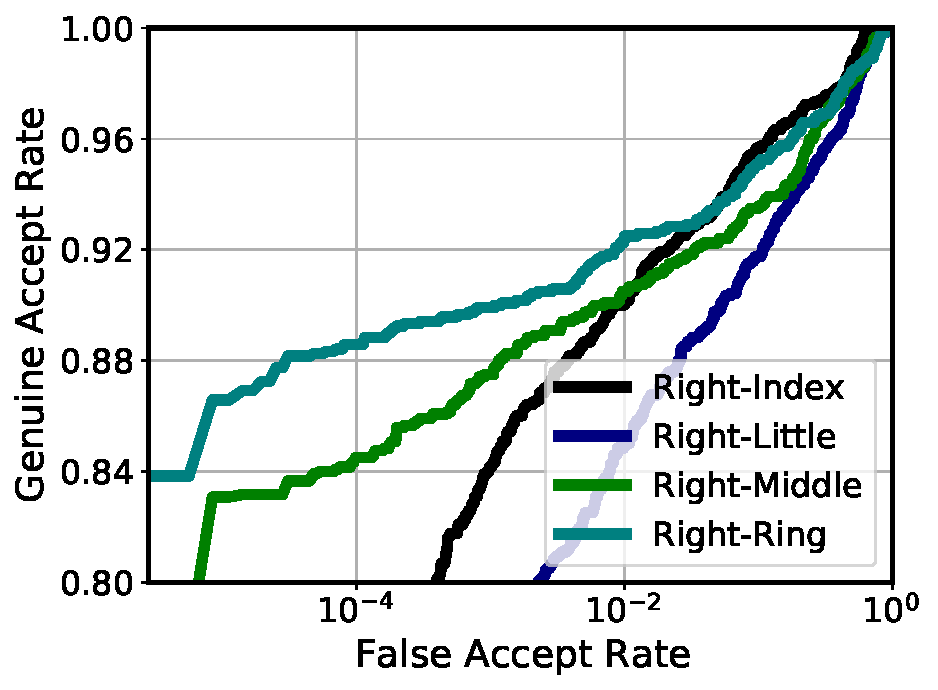
\includegraphics[width=3in]{Figure/15-10-2022/trained-roc.pdf}}
    \caption{Comparative ROC curve from using little knuckle, ring finger knuckle, middle finger knuckle, and index finger knuckle of right hand}
    \label{trained}
\end{figure*}



\subsection{Plans}
\begin{itemize}
    \item I will also use the graph neural network to encoding the finger knuckle keypoints graph. In this method, the finger nail blood vessel keypoints can also use the graph neural network. As for the method how to detect the keypoints of finger knuckle, I will try to use the SuperPoint \cite{detone2018superpoint} model to detect.
    \item  If the accuracy of graph neural network can get a good results on finger knuckle, I will also try to implement it on fingerprint identification task.
    \item I will change the score fusion method to MLP network.
\end{itemize} 


\section{Fingernail Blood Vessel Recognition by Key Points}

\subsection{A Comprehensive Survey on Graph Neural Network \cite{wu2020comprehensive}}

The paper uses a new taxonomy of GNNs. GNNs are categorized into four groups: recurrent GNNs (RecGNN), convolutional GNNs (ConvGNNs), graph autoencoders (GAEs), and spatial-temporal GNNs (STGNNs). At for the STGNNs, it just a variance of a normal GNNs, because it adds a time series which the GNNs' attribute will change with time based on the normal graph.

\textcolor{red}{\subsection{What I have Done}}
I use the detected keypoints as nodes to compose the graph. I first select a part of the keypoints from the detected files and then sort them by confidence. The sorted nodes are connected sequentially to form the graph. The characteristics of each node are $(x, y, angle, class, confidence)$, and the weight of each edge is the same. As for the message passing function, I use the formula ${x}^{\prime}_i = \mathbf{W}_1 \mathbf{x}_i + \mathbf{W}_2\sum_{j \in \mathcal{N}(i)} e_{j,i} \cdot \mathbf{x}_j$ to calculate the current node state with its neighbor nodes. And I am training it as a classification task, and the result is which category this graph belongs to. I divided a total of 84 test data into training data, validation data, and test data in the ratio 8:1:1. Form the Fig. \ref{network}, it is the forwarding function of my graph neural network.

\begin{figure*}[ht!]
    \centering
    \subfloat[]{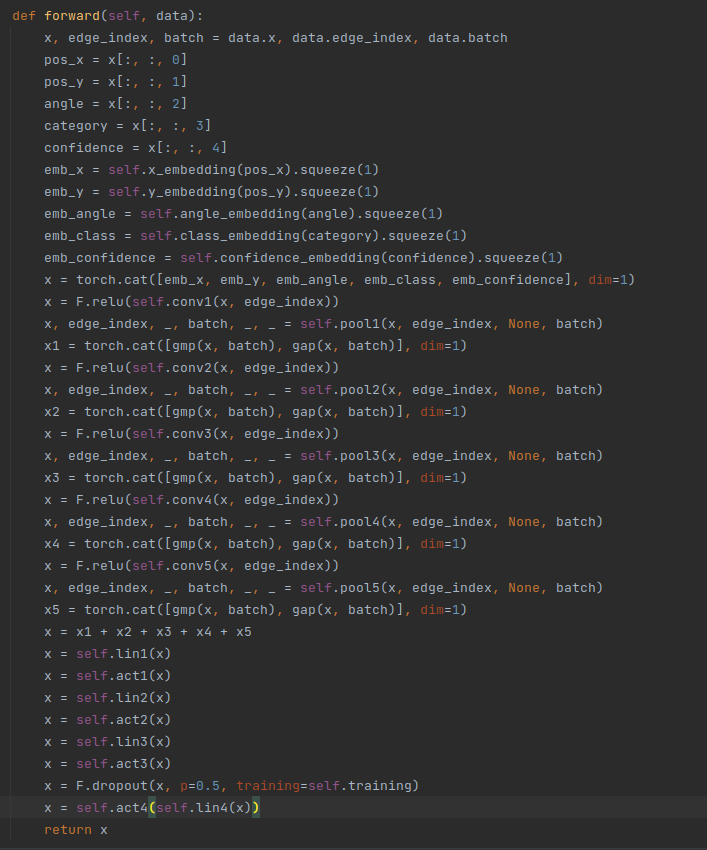
\includegraphics[width=3in]{Figure/15-10-2022/network.png}}
    \caption{the forwarding function of my graph neural network}
    \label{network}
\end{figure*}


\subsubsection{Using 128 Ending Points}
\begin{figure*}[ht!]
    \centering
    \subfloat[]{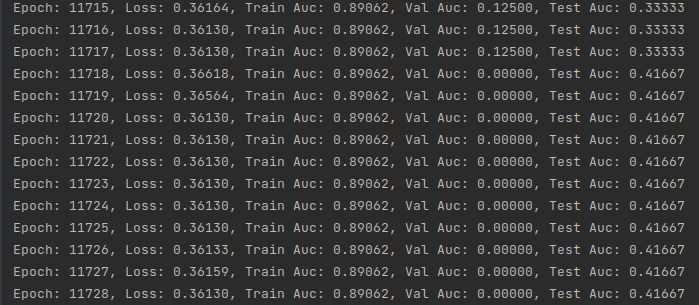
\includegraphics[width=3in]{Figure/15-10-2022/ending-128.png}}
    \caption{the training accuracy and testing accuracy by training 128 ending points}
    \label{ending-128}
\end{figure*}

From the Fig. \ref{ending-128}, the accuracy on the training set can get 0.89062, while the accuracy on the testing set just is 0.41667. In this kind of situation, the prediction accuracy is too low.

\subsubsection{Using 32 Ending Points}
When I only use 32 ending points to compose a graph as the input data for training graph neural network. Because the accuracy when I use 128 ending points to compose graph is too low, the result of 32 ending points is lower than the 128 ending points.


\subsection{Plans}
When I choose bifurcation as the node to form the graph, my code reports an error. Or if I input too many nodes, my code also reports an error. \textcolor{red}{Next step should solve these problems firstly.} The key problem of graph neural network is how to construct the edge information of a graph, and another one is how to construct the message passing function. In my above experiments, I simply built the graph with each node connected at the beginning and end, and with the same weight for each edge. 
\begin{itemize}
    \item Changing my current graph neural network because of low accuracy
    \item Using different method to link the ending points and bifurcation as graph edges
    \item Using different message passing function to get better result
\end{itemize}




\section{Reproduce Iris Recognition of Eddie}

The segmentation step of the Iris dataset has been completed, and the other steps have not yet been started.

\subsection{Plans}
Follow the steps in the paper to continue with the Iris identification of the headwear dataset.


